\documentclass{beamer}

\usepackage[utf8]{inputenc}

\title{Sandsynlighedsteori og Lineær algebra}
\subtitle{Workshop 4 - Linear optimization}
\author{Sebastian Livoni Larsen}

\usepackage{tikz}
\usepackage{pgfplots,pgfplotstable}
\pgfplotsset{compat=1.15}

\begin{document}
	\frame {
		\titlepage
	}

  \frame{
    \frametitle{Sparse solutions to linear algebraic systems}
    \framesubtitle{\textbf{Exercise 1} - Explain why the objective function does not satisfy the definition of a linear tranformation.}

    \begin{align*}
      f(x)=\sum_{i=1}^n|x_i| \\
      -1 \cdot f(x) \neq f(-1\cdot x) \\
      -1 \cdot f(1) = -1 \\
      f(-1 \cdot 1) = 1 \\
      \text{Hence, }-1\cdot f(1) \neq f(-1 \cdot 1)
    \end{align*}
  }

  %\frame{
  %  \frametitle{Sparse solutions to linear algebraic systems}
  %  \framesubtitle{\textbf{Exercise 2} - }
  %}

  \frame{
    \frametitle{Sparse solutions to linear algebraic systems}
    \framesubtitle{\textbf{Exercise 3} - Determining all 10 basic solutions and select out of them 5 feasible basic solutions}
    \fontsize{5pt}{7.2}\selectfont

    \begin{align*}
      \tilde{A}\tilde{x}=b \\
      \begin{bmatrix}
        1 & 2 & 3 & 4 & 5 & -1 & -2 & -3 & -4 & -5
      \end{bmatrix}
      \tilde{x}=\begin{bmatrix}
        10
      \end{bmatrix}
    \end{align*}
    The 10 basic solutions are therefore:
    \begin{align*}
      \tilde{A}
        \begin{bmatrix}
          x_1 & 0 & 0 & 0 & 0 & 0 & 0 & 0 & 0 & 0
        \end{bmatrix}^T
        =
        \begin{bmatrix}10\end{bmatrix},\qquad s_1=\begin{bmatrix}
          \frac{10}{1} & 0 & 0 & 0 & 0 & 0 & 0 & 0 & 0 & 0
        \end{bmatrix} \\
        \tilde{A}
        \begin{bmatrix}
          0 & x_2 & 0 & 0 & 0 & 0 & 0 & 0 & 0 & 0
        \end{bmatrix}^T
        =
        \begin{bmatrix}10\end{bmatrix},\qquad s_2=\begin{bmatrix}
          0 & \frac{10}{2} & 0 & 0 & 0 & 0 & 0 & 0 & 0 & 0
        \end{bmatrix} \\
        \tilde{A}
        \begin{bmatrix}
          0 & 0 & x_3 & 0 & 0 & 0 & 0 & 0 & 0 & 0
        \end{bmatrix}^T
        =
        \begin{bmatrix}10\end{bmatrix},\qquad s_3=\begin{bmatrix}
          0 & 0 & \frac{10}{3} & 0 & 0 & 0 & 0 & 0 & 0 & 0
        \end{bmatrix} \\
        \tilde{A}
        \begin{bmatrix}
          0 & 0 & 0 & x_4 & 0 & 0 & 0 & 0 & 0 & 0
        \end{bmatrix}^T
        =
        \begin{bmatrix}10\end{bmatrix},\qquad s_4=\begin{bmatrix}
          0 & 0 & 0 & \frac{10}{4} & 0 & 0 & 0 & 0 & 0 & 0
        \end{bmatrix} \\
        \tilde{A}
        \begin{bmatrix}
          0 & 0 & 0 & 0 & x_5 & 0 & 0 & 0 & 0 & 0
        \end{bmatrix}^T
        =
        \begin{bmatrix}10\end{bmatrix},\qquad s_5=\begin{bmatrix}
          0 & 0 & 0 & 0 & \frac{10}{5} & 0 & 0 & 0 & 0 & 0
        \end{bmatrix} \\
        \tilde{A}
        \begin{bmatrix}
          0 & 0 & 0 & 0 & 0 & x_6 & 0 & 0 & 0 & 0
        \end{bmatrix}^T
        =
        \begin{bmatrix}10\end{bmatrix},\qquad s_6=\begin{bmatrix}
          0 & 0 & 0 & 0 & 0 & \frac{10}{-1} & 0 & 0 & 0 & 0
        \end{bmatrix} \\
        \tilde{A}
        \begin{bmatrix}
          0 & 0 & 0 & 0 & 0 & 0 & x_7 & 0 & 0 & 0
        \end{bmatrix}^T
        =
        \begin{bmatrix}10\end{bmatrix},\qquad s_7=\begin{bmatrix}
          0 & 0 & 0 & 0 & 0 & 0 & \frac{10}{-2} & 0 & 0 & 0
        \end{bmatrix} \\
        \tilde{A}
        \begin{bmatrix}
          0 & 0 & 0 & 0 & 0 & 0 & 0 & x_8 & 0 & 0
        \end{bmatrix}^T
        =
        \begin{bmatrix}10\end{bmatrix},\qquad s_8=\begin{bmatrix}
          0 & 0 & 0 & 0 & 0 & 0 & 0 & \frac{10}{-3} & 0 & 0
        \end{bmatrix} \\
        \tilde{A}
        \begin{bmatrix}
          0 & 0 & 0 & 0 & 0 & 0 & 0 & 0 & x_9 & 0
        \end{bmatrix}^T
        =
        \begin{bmatrix}10\end{bmatrix},\qquad s_9=\begin{bmatrix}
          0 & 0 & 0 & 0 & 0 & 0 & 0 & 0 & \frac{10}{-4} & 0
        \end{bmatrix} \\
        \tilde{A}
        \begin{bmatrix}
          0 & 0 & 0 & 0 & 0 & 0 & 0 & 0 & 0 & x_{10}
        \end{bmatrix}^T
        =
        \begin{bmatrix}10\end{bmatrix},\qquad s_{10}=\begin{bmatrix}
          0 & 0 & 0 & 0 & 0 & 0 & 0 & 0 & 0 & \frac{10}{-5}
        \end{bmatrix} \\
    \end{align*}
    $s_6, s_7, s_8, s_9, s_{10}$ are not feasible solutions because they contains negative entries. Therefore the remaining $s_1, s_2, s_3, s_4, s_5$ are feasible solutions with the best solution being $s_5$ because: \[\frac{10}{5} < \frac{10}{4} < \frac{10}{3} < \frac{10}{2} < \frac{10}{1}\]
  }

  \frame{
    \frametitle{Sparse solutions to linear algebraic systems}
    \framesubtitle{\textbf{Exercise 4} - Converting the problem (\ref{prob:LP2}) to a linear optimization problem in canonical form}

    \begin{equation}\label{prob:LP2}\begin{aligned}
      &\text{minimize} && \tilde{c}\cdot \tilde{x},\\
      &\text{subject to}&&\\
      &&&\tilde{A}\tilde{x}= b,\\
      &&& \tilde{x}\geq 0.
    \end{aligned}\end{equation}

    Converted to canonical form:
    \begin{align*}
      \begin{aligned}
        &\text{maximize} && -\tilde{c}\cdot \tilde{x},\\
        &\text{subject to}&&\\
        &&&\tilde{A}\tilde{x} \leq b,\\
        &&&-\tilde{A}\tilde{x} \leq -b, \\
        &&& \tilde{x}\geq 0.
      \end{aligned}
    \end{align*}
  }

  \frame{
    \frametitle{Sparse solutions to linear algebraic systems}
    \framesubtitle{\textbf{Exercise 5} - Writing down the dual problem for the linear optimization problem in canonical form.}

    Converted to canonical form:
    \begin{align*}
      \begin{aligned}
        &\text{maximize} && -\tilde{c}\cdot \tilde{x},\\
        &\text{subject to}&&\\
        &&&\tilde{A}\tilde{x} \leq b,\\
        &&&-\tilde{A}\tilde{x} \leq -b, \\
        &&& \tilde{x}\geq 0.
      \end{aligned}
    \end{align*}

    Converting it into a dual problem:
    \begin{align*}
      \begin{aligned}
        &\text{minimize} && b\cdot y_1-b \cdot y_2,\\
        &\text{subject to}&&\\
        &&&\begin{bmatrix}\tilde{A} \\ -\tilde{A}\end{bmatrix}^Ty \geq -\tilde{c}\\
        &&& y \geq 0.
      \end{aligned}
    \end{align*}
  }

  \frame{
    \frametitle{Sparse solutions to linear algebraic systems}
    \framesubtitle{\textbf{Exercise 5} - Sketching the feasible set for the dual problem and solve it graphically (continuation).}

    The feasible set sketched is:
    \begin{align*}
      \begin{aligned}
        &\text{minimize} && \begin{bmatrix}10\end{bmatrix} \cdot y_1-\begin{bmatrix}10\end{bmatrix}  \cdot y_2,\\
        &\text{subject to}&&\\
        &&& \begin{bmatrix}
          1 & -1 \\ 2 & -2 \\ 3 & -3 \\ 4 & -4 \\ 5 & -5 \\ -1 & 1 \\ -2 & 2 \\ -3 & 3 \\ -4 & 4 \\ -5 & 5
        \end{bmatrix}y \geq \begin{bmatrix}
          -1 \\-1 \\-1 \\-1 \\-1 \\-1 \\-1 \\-1 \\-1 \\-1
        \end{bmatrix} \\
        &&& y \geq 0.
      \end{aligned}
    \end{align*}
  }

  \frame{
    \frametitle{Sparse solutions to linear algebraic systems}
    \framesubtitle{\textbf{Exercise 5} - Sketching the feasible set for the dual problem and solve it graphically (continuation). Do we obtain the same optimal value as in question 3?}

    \begin{figure}[htb]
      \centering
      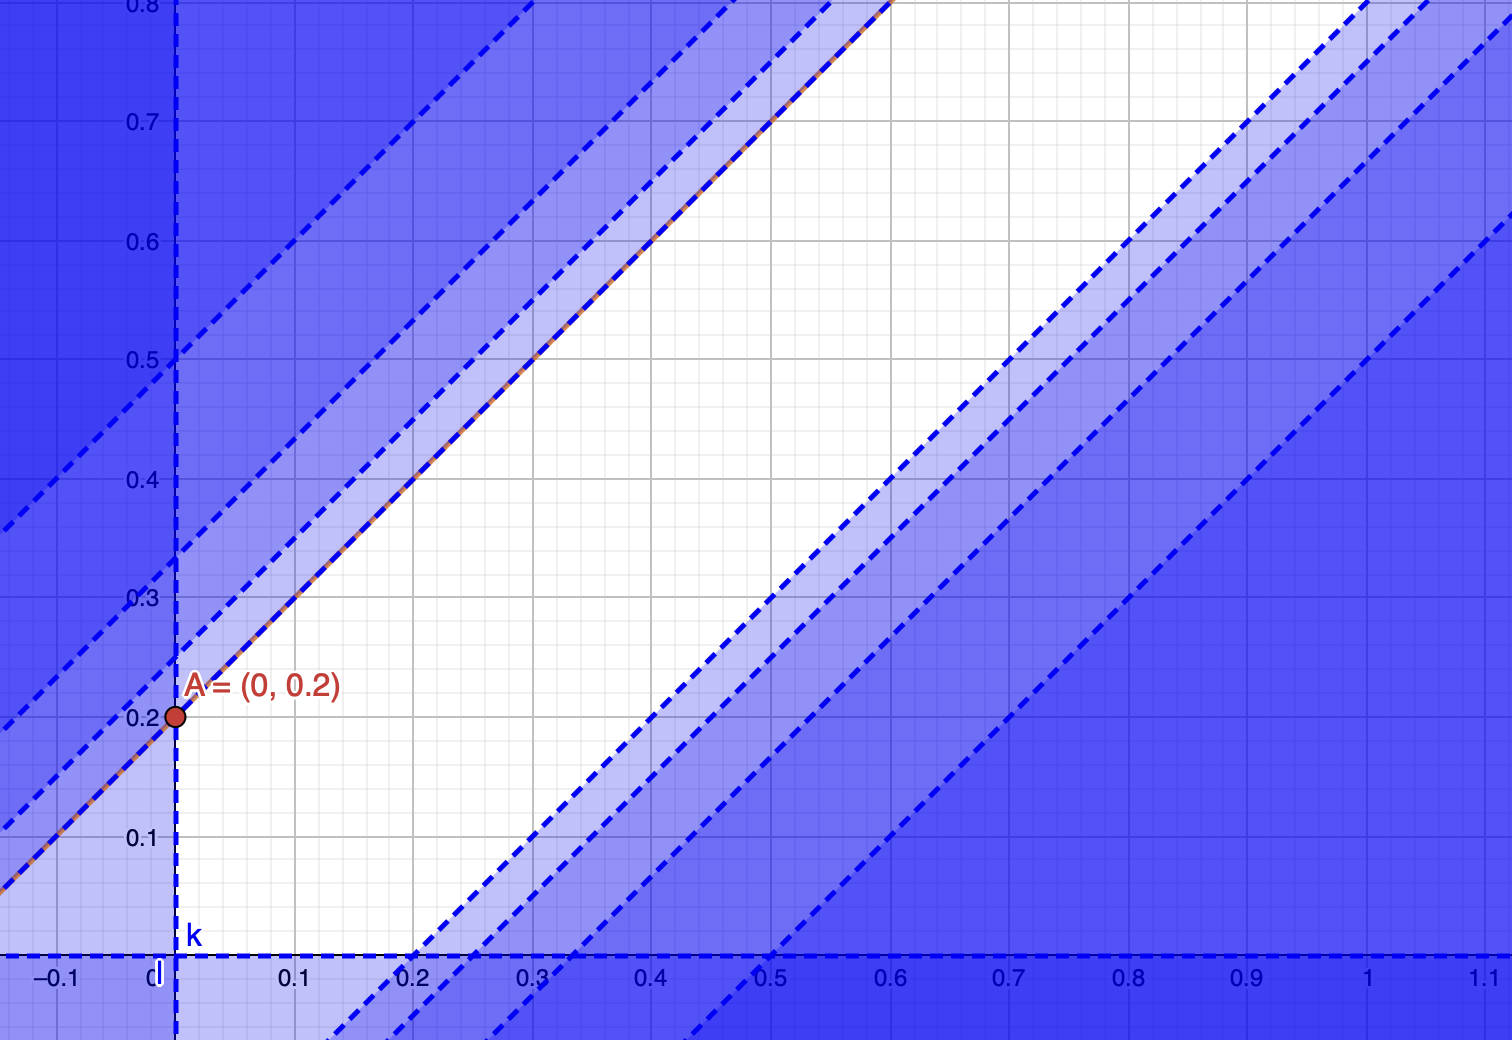
\includegraphics[width=0.8\textwidth]{assets/feasible_set_exercise_5.png}
    \end{figure}

    \begin{itemize}
      \item We obtain the value $10 \cdot 0 - 10 \cdot 0.2 = -2$.
      \item Yes, we obtain the same value: $-(-2)=2$.
    \end{itemize}

  }

  
  
\end{document}